\subsection{Giao diện quản lý yêu cầu từ thành viên trong workspace}

\begin{figure}[H]
    \centering
    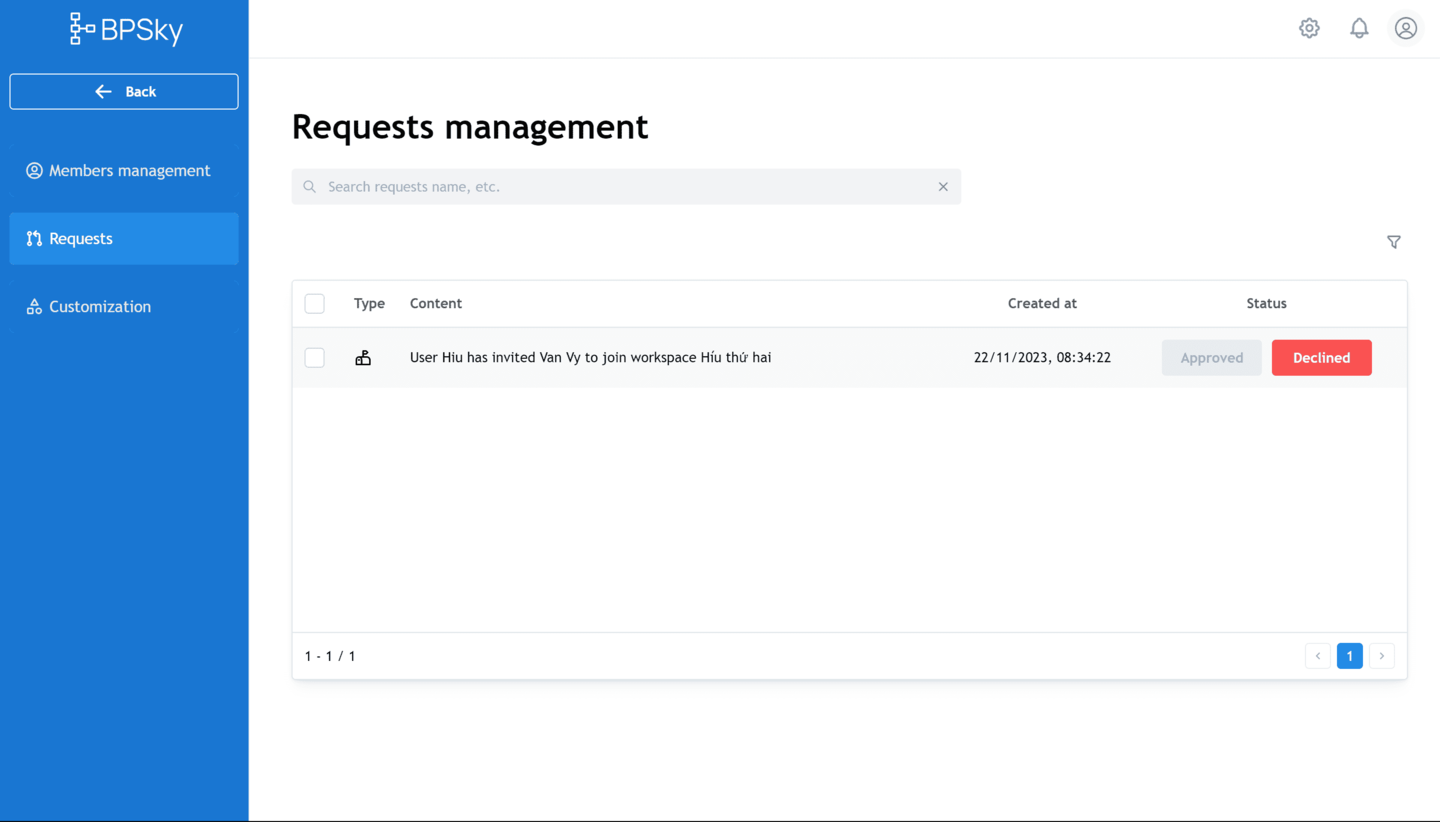
\includegraphics[ width = 0.8\linewidth]{Content/Hiện thực hệ thống/documents/Hiện thực giao diện người dùng/images/RequestsManagementPage.png}
    \vspace{0.5cm}
    \caption{Giao diện trang quản lý yêu cầu từ thành viên trong workspace}
    \label{fig: Giao diện trang quản lý yêu cầu từ thành viên trong workspace}
\end{figure}

\begin{figure}[H]
    \centering
    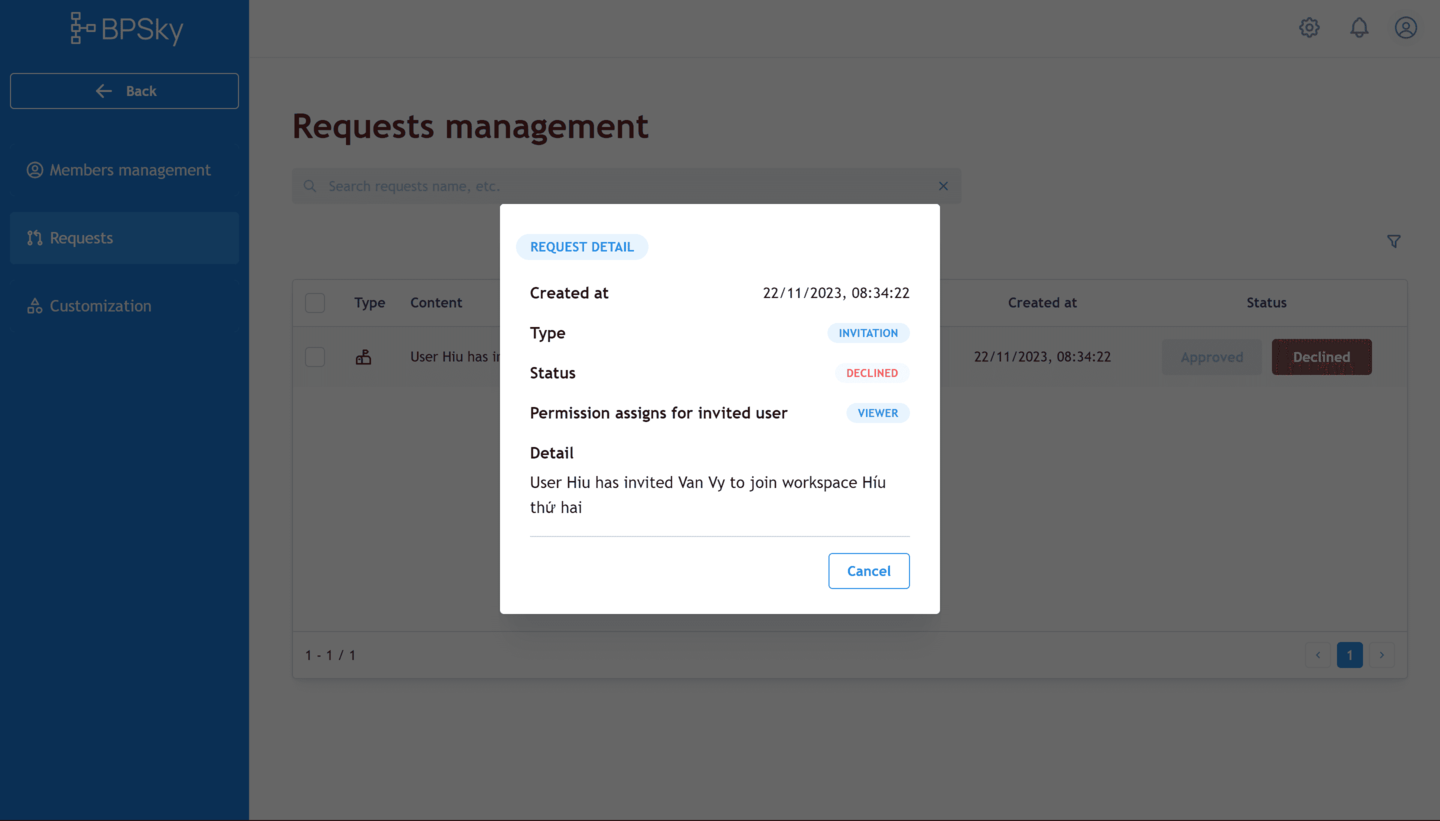
\includegraphics[ width = 0.8\linewidth]{Content/Hiện thực hệ thống/documents/Hiện thực giao diện người dùng/images/RequestDetailModal.png}
    \vspace{0.5cm}
    \caption{Giao diện modal hiển thị thông tin chi tiết của yêu cầu}
    \label{fig: Giao diện modal hiển thị thông tin chi tiết của yêu cầu}
\end{figure}

Khi người dùng chọn "Request management" ở thanh sidebar thì hệ thống sẽ chuyển hướng người dùng tới trang quản lý yêu cầu của workspace. Tại đây, hệ thống sẽ hiển thị danh sách những yêu cầu được gửi từ phía thành viên bên trong workspace. Các yêu cầu từ phía thành viên sẽ được phân thành 2 loại: Yêu cầu điều chỉnh vai trò trong workspace và Yêu cầu mời thành viên bên ngoài vào workspace. Người dùng có thể chọn "Approve" hoặc "Decline" để phản hồi yêu cầu tương ứng. Nếu người dùng muốn xem thông tin chi tiết của yêu cầu, người dùng có thể nhấn vào item yêu cầu tương ứng, hệ thống sẽ hiển thị modal như hình \ref{fig: Giao diện modal hiển thị thông tin chi tiết của yêu cầu}.